

\documentclass{article}        % Your input file must contain these two lines 
\usepackage{bm}
\usepackage{graphicx}
\usepackage{subfigure}
\usepackage{amsmath}
\usepackage{esint}

\title{A note about solving the fracture flow problem by the finite volume method (FVM)}
\author         {Tingchang Yin \\School of Engineering, Westlake University, Hangzhou, China\\yintingchang@foxmail.com}

\date{\today}  
    


\begin{document}               % plus the \end{document} command at the end.
\maketitle
\begin{abstract}
	FVM on unstructured mesh. 
\end{abstract}
\section{Governing laws}
The governing equation is
\begin{equation}
k\bm{\Delta} h + F = 0, 
\end{equation}
where $h$ is the hydraulic head, $k$ is the fracture conductivity (here it is assumed to be isotropic), and $F$ is the source term.

\section{Control volume}
Let $\Omega$ denotes the fracture domain, and a mesh consisting of triangles is generated. The vertices of triangles are the nodes storing the head field. One node has a control volume, $\Delta V$. An example is shown in Fig. \ref{controlvolume}. Generally, the volume is a polygon enclosed by the circumcenters of the triangles sharing the node. However, if thin triangle exists, the circumcenter could be outside the triangle. Here, I use the barycenter of triangles.

\begin{figure}[htb]
	\centering
	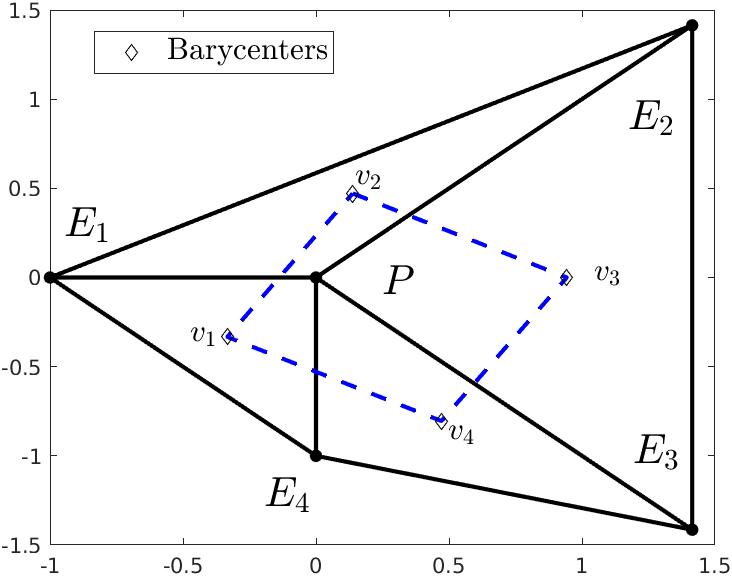
\includegraphics[scale=0.4]{figures/control_volume.png}
	\caption{The control volume of a node $P$.}
	\label{controlvolume}
\end{figure} 

Let us integrate the governing equation over $\Delta V$:
\begin{equation}
k \int_{\Delta V}\bm{\Delta} h \mathrm{d}V + \int_{\Delta V}F \mathrm{d}V = 0.
\label{integrate_poisson}
\end{equation}
By using the Green's formula, the Eq. (\ref{integrate_poisson}) can be rewritten as
\begin{equation}
k\oint_{S_{\Delta V}} \bm{n}\cdot \bm{\nabla} h \mathrm{d}S + \bar{F}{\Delta V} = 0,
\label{surface_integrate}
\end{equation}
where $S_{\Delta V}$ is the surfaces of $\Delta V$, and $\bm{n}$ is the inward normal vectors of the surfaces. Let $N_e$ denotes the number of edges of $\Delta V$, and Eq. (\ref{surface_integrate}) can be further rewritten as
\begin{equation}
k\sum_{g = 1}^{N_e}A_g\cdot \bm{n}_g \cdot \bm{\nabla}h + \bar{F}{\Delta V} = 0,
\label{sum_flux}
\end{equation} 
where $A_g$ is the surface area of the $g$th edge, and $n_g$ is the inward normal vector. This equation hints that the flux is conserved over the $\Delta V$, because $\bm{\nabla}h$ is actually the vectorial flux rate. Besides, $\bm{n}_g \cdot \bm{\nabla}h = \frac{\partial h}{\partial n}$ that is the scalar flux rate along the normal vector. 

Let us ten discretize the Eq. (\ref{sum_flux}). The Fig. \ref{controlvolume} is taken as an example. Let us consider the flux through the edge $v_1,v_2$ first, which is
\begin{equation}
A_{1} \cdot {q_{\perp 1}}, \notag
\end{equation}
and ${q_{\perp 1}}$ is the scalar flux rate perpendicular to the edge $v_1,v_2$. Let $\theta_{1}$ is the angle between the outward normal vector of edge $v_1,v_2$ and edge $E_1, P$, and hence we have
\begin{equation}
{q_{\perp 1}} = {q_{E_1, P}} \cdot \cos{\theta_{1}}, \notag
\end{equation}
where ${q_{E_1, P}}$ is the scalar flux rate along edge $E_1, P$. The  ${q_{E_1, P}}$ can be approximated by
\begin{equation}
	k\cdot \frac{h_{E_1} - h_P}{l_{E_1, P}}, \notag
\end{equation}
and $l_{E_1, P}$ is the length of the edge ${E_1, P}$. Therefore, the overall flux through edge $v_4,v_1$ is
\begin{equation}
	A_{1} \cdot 	k\cdot \frac{h_{E_1} - h_P}{l_{E_1, P}} \cdot \cos{\theta_{1}}. \notag	
\end{equation}
In a similar way, the flux through other edges of $\Delta V$ can be calculated and finally the Eq. (\ref{sum_flux}) can be discretized into
\begin{equation}
k\sum_{r = 1}^{N_e}A_{r}\cdot \frac{h_{r} - h_P}{l_{E_r, P}}\cdot \cos{\theta_{r}} + \bar{F}\cdot \Delta V = 0.
\label{discrete_} 
\end{equation}
Let us sort this equation: for node $P$ (or $h_P$), the coefficient is given by
\begin{equation}
\alpha_P = k\sum_{r = 1}^{N_e}A_{r}\cdot \frac{-1}{l_{E_r, P}}\cdot \cos{\theta_{r}}, 
\end{equation}
and for each node connecting to $P$, the coefficient is
\begin{equation}
\alpha_r = k \cdot A_{r}\cdot \frac{1}{l_{E_r, P}}\cdot \cos{\theta_{r}}, r \in [1, N_e].
\end{equation}
The source term is generally linearized:
\begin{equation}
\bar{F}\cdot \Delta V = F_u + F_P\cdot h_P,
\end{equation}
and so, the simplified form of Eq. (\ref{discrete_}) is
\begin{equation}
\left(-\alpha_P -F_P\right) h_P = \sum\alpha_r\cdot h_{E_r} + F_u,
\end{equation}
where $r \in [1, N_e]$. If $F$ is a constant, then $F_u = F$ and $F_p = 0$.

\section{Control volume of boundary nodes}
The control volume of a boundary node is shown in Fig. \ref{boundary_control_volume}. $P$ is the boundary node and the polygon $v_1, v_2, v_3, v_4, P$ is the control volume.

\begin{figure}[htb]
	\centering
	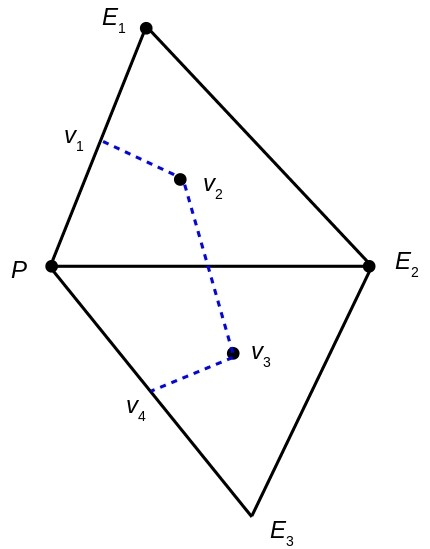
\includegraphics[scale=0.4]{figures/BC_control_volume.jpg}
	\caption{A boundary node and the control volume.}
	\label{boundary_control_volume}
\end{figure}

First, let us talk about the Dirichlet boundary condition which is given by
\begin{equation}
	h_D = C, \text{ on } \Gamma_D,
\end{equation}
where $C$ is a constant value. In this circumstance, we do not have to establish a control volume, and we just have
\begin{equation}
	h_P = C.
\end{equation}

Given that the Neumann boundary condition is
\begin{equation}
\bm{n}\cdot \nabla h = 0,
\end{equation}
and that means the normal flux rate though the edge is zero. Let us raise an example: in Fig. \ref{boundary_control_volume}, edges $E_1, P$ and $E_3, P$ are both of Neumann boundaries. The edges $v_1, P$ and $v_4, P$ are impervious, and so, we have
\begin{equation}
	\alpha_P = k\sum_{r = 1}^{3}A_r \cdot \frac{-1}{l_{E_r, P}}\cdot \cos{\theta_r},
\end{equation}
and
\begin{equation}
	\alpha_r = k \cdot A_{r}\cdot \frac{1}{l_{E_r, P}}\cdot \cos{\theta_{r}}, r \in [1, 3]. 
\end{equation}
$F_p$ and $F_u$ are both zero.

 
\end{document}

